\begin{frame}[fragile]{\shortt: Experimento, Quilombo}
\begin{center}
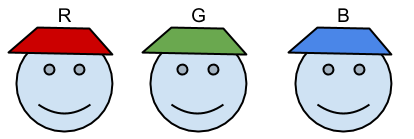
\includegraphics[scale=0.3]{images/caras1.png}
\end{center}
\bigskip

\only<1>{
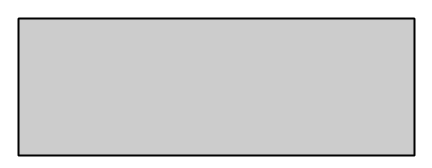
\includegraphics[scale=0.3]{images/fondo1.png}

\includegraphics[scale=0.3]{images/fondo2.png}
}

\only<2>{
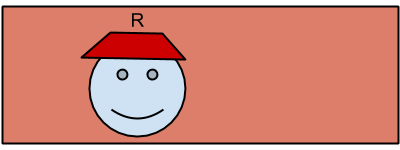
\includegraphics[scale=0.3]{images/h1.png}
}

\only<3>{
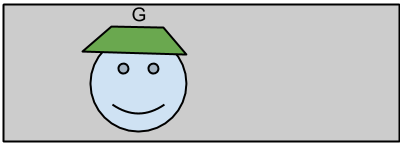
\includegraphics[scale=0.3]{images/h2.png}
}

\only<4>{
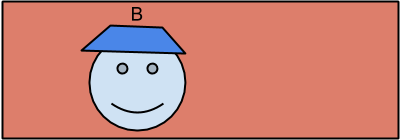
\includegraphics[scale=0.3]{images/h3.png}
}

\only<5>{
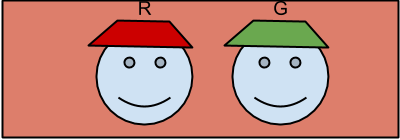
\includegraphics[scale=0.3]{images/h4.png}
}

\only<6>{
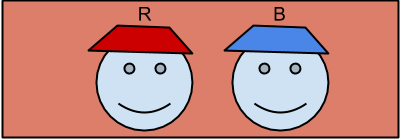
\includegraphics[scale=0.3]{images/h5.png}
}

\only<7>{
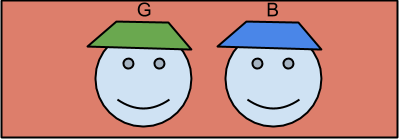
\includegraphics[scale=0.3]{images/h6.png}
}

\only<8>{
\begin{center}
    Para escribir en su hoja: Cuál de los sujetos consideran quilomberos?
\end{center}
}


\end{frame}